\documentclass{article}[12pt]

%--------------Packages------------------------------
\usepackage[utf8]{inputenc} %Pour encoder du texte en français
\usepackage[francais]{babel} %Pour encoder du texte en français
\usepackage{graphicx} %pour inclure des images
\usepackage{version} % permet d'utiliser l'environnement comment
\graphicspath{{./figures/}} %repertoire images
\usepackage{listings} %si on veut afficher du code, le code doit se trouver dans un dossier "codes" 					  %lui même dans le même répertoire que ce fichier tex
\usepackage{color} %nécessaire pour changer les couleurs du highlighting du code
\usepackage{amsmath,amssymb}%pour des maths au cas où
\usepackage{array,multirow,makecell}%Pour manipuler les tableaux
\usepackage{url} %pour utiliser les liens hypertextes
\usepackage{hyperref} %pour utiliser les liens hypertextes
\usepackage{float}
\usepackage{glossaries}
\makeglossaries 
\newlength{\length}
\setlength{\length}{3\baselineskip}

% ---------- Document ------------ %
\begin{document}
\newacronym{RFE}{RFE}{Request For Enhancement}
\newacronym{PointClick}{Point \& Click}{Pointer \& Cliquer }
\begin{titlepage}

\newcommand{\HRule}{\rule{\linewidth}{0.5mm}} % Defines a new command for the horizontal lines, change thickness here

\center % Center everything on the page
 
%----------------------------------------------------------------------------------------
%	HEADING SECTIONS
%----------------------------------------------------------------------------------------

\textsc{\LARGE Institut Paul Lambin}\\[1.5cm] % Name of your university/college
\textsc{\Large BAC 2 Informatique de gestion}\\[0.5cm] % Major heading such as course name
\textsc{\large Ergonomie Web}\\[0.5cm] % Minor heading such as course title

%----------------------------------------------------------------------------------------
%	TITLE SECTION
%----------------------------------------------------------------------------------------

\HRule \\[0.4cm]
{ \huge \bfseries Ergonomie Web - Travail 4 }\\[0.4cm] % Title of your document
\HRule \\[1.5cm]
 
%----------------------------------------------------------------------------------------
%	AUTHOR SECTION
%----------------------------------------------------------------------------------------

\begin{minipage}{0.4\textwidth}
\begin{flushleft} \large
\emph{Auteurs:}\\
Christopher \textsc{Sacré} \\
Damien \textsc{Meur} % Your name
\end{flushleft}
\end{minipage}
~
\begin{minipage}{0.4\textwidth}
\begin{flushright} \large
\emph{Professeur:} \\
D. \textsc{Grolaux} % Supervisor's Name
\end{flushright}
\end{minipage}\\[4cm]

% If you don't want a supervisor, uncomment the two lines below and remove the section above
%\Large \emph{Author:}\\
%John \textsc{Smith}\\[3cm] % Your name

%----------------------------------------------------------------------------------------
%	DATE SECTION
%----------------------------------------------------------------------------------------

{\large \today}\\[3cm] % Date, change the \today to a set date if you want to be precise

%----------------------------------------------------------------------------------------
%	LOGO SECTION
%----------------------------------------------------------------------------------------

%\includegraphics{Logo}\\[1cm] % Include a department/university logo - this will require the graphicx package
 
%----------------------------------------------------------------------------------------

\vfill % Fill the rest of the page with whitespace

\end{titlepage}

\tableofcontents%table des matières
\newpage


%différentes sections
\section{Présentation du site}
\subsection{URL}
\url{http://www.tennisclubdeparis.fr/}
\subsection{Présentation du site}
\begin{figure}[H]
	\centering    \fbox{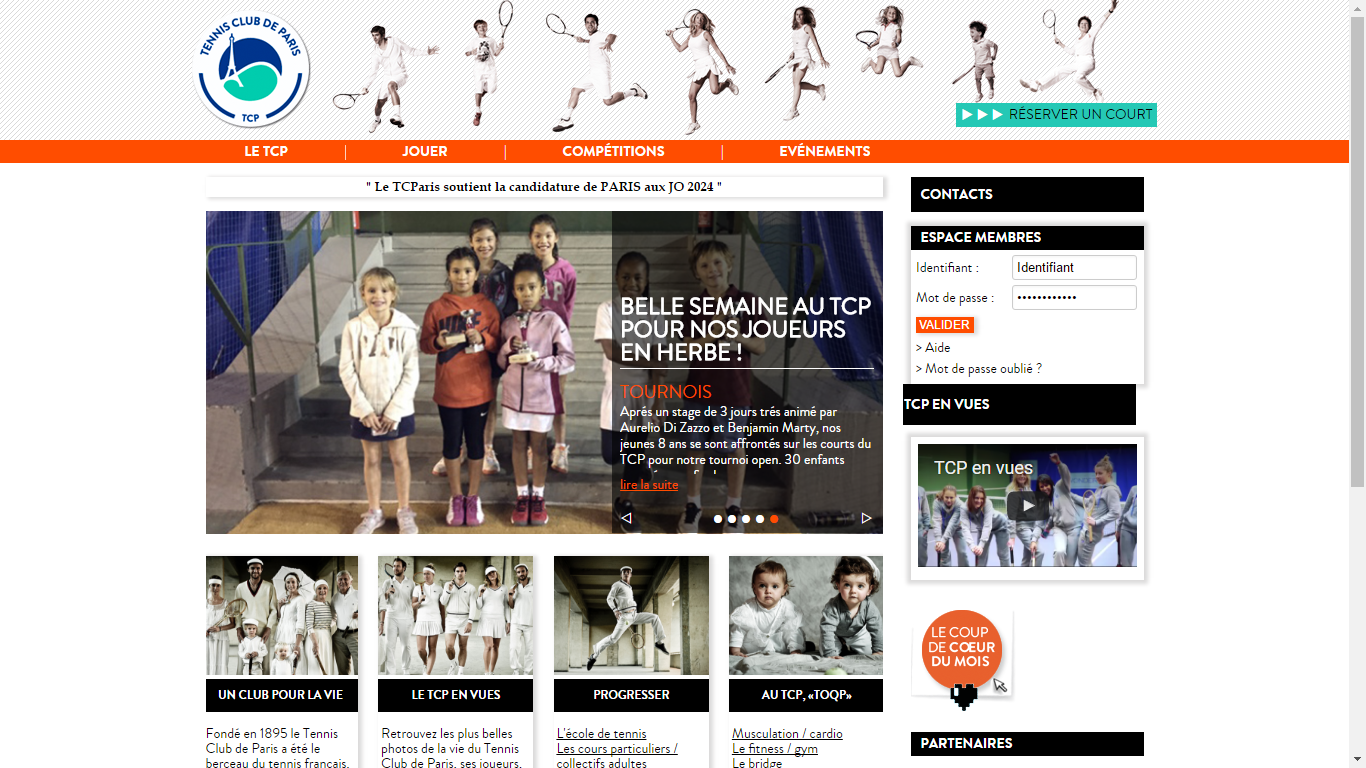
\includegraphics[width=\textwidth, height=10cm]{main.png}}
    \caption{Page d'accueil du site}
\end{figure}
\begin{itemize}
	\item Site pour un club de tennis
    \item Brève présentation du club et de ses différentes catégories de joueurs
    \item Possibilité de réserver un cours
    \item Possibilité de voir les prochain tournois / compétitions
    \item Possibilité de voir les événements passés du club
\end{itemize}
\section{Techniques des cartes à trier}
\begin{figure}[H]
	\centering   \fbox{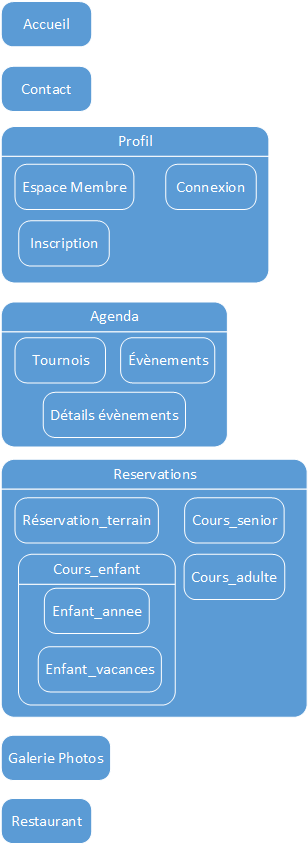
\includegraphics[height=16cm]{cartes.png}}
\end{figure}
\textcolor{red}{\textbf{Question Christopher} : On n'essaierait pas de placer les fenêtres un peu horizontalement pour que l'image prenne mois de place verticalement ? Comme ça on peut décrire ce qui a dedans en une seule page.}
\section{Évaluation du site par les utilisateurs}
\begin{figure}[H]
	\centering   \fbox{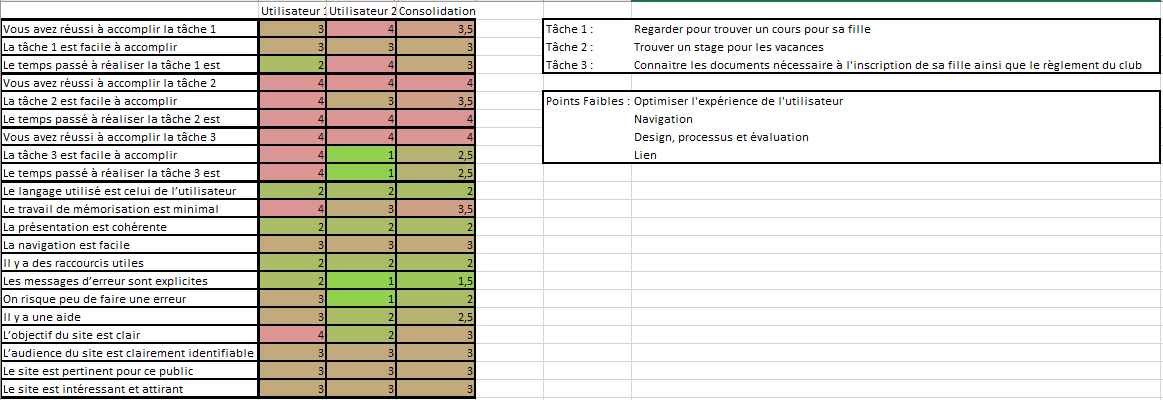
\includegraphics[width=\textwidth, height=6cm]{eval_utils.PNG}}
\end{figure}
Pour l'évaluation du site, nous nous sommes identifiés au personna \textit{Tsao Ming} créé dans notre précédent travail. \textit{Tsao Ming} est une mère célibataire de 37 ans qui veut trouver un nouveau club de tennis pour ses enfants. Nous avons défini 3 tâches à accomplir qui répondent à son profil :
\begin{enumerate}
	\item Trouver un cours pour sa fille (pour l'année scolaire).
	\item Trouver un stage pour sa fille (pour les vacances scolaires).
	\item Trouver les documents nécessaires à l'inscription de sa fille (y compris le règlement du club).
\end{enumerate}
Nous discuterons dans la section \ref{prob_important} des principaux problèmes d'ergonomie rencontrés durant notre navigation sur le site lors de la réalisation de ces objectifs.
\newpage
\section{Problèmes ergonomiques importants}
\label{prob_important}
\subsection{L'expérience utilisateur}
En arrivant sur le site, on constate directement une fenêtre de connexion à un espace membre. Nous n'avons malheureusement pas pu nous inscrire sur celui-ci, car si la connexion se fait depuis le site, l'inscription elle se fait par e-mail, nous reviendrons sur ce problème d'ergonomie et la règle du code d'ergonomie  \footnote{SCHEIDERMAN B et LEAVITT 0.M. \textit{Research-Based Web Design \& Usability Guidelines.} GSA.  Washigton, USA.} qu'il enfreint dans la sous-section \ref{work-load}. 
\subsection{Contenu}
Le site permet sans doute de visualiser davantage de contenu lors de la connexion à son espace membre, mais il aurait été utile d'expliquer les avantages / fonctionnalités de celle-ci, un utilisateur quidam (comme notre personna) peut difficilement comprendre avec le peu d'information qui lui est présenté doit peut être mise en complément de cette lourde tâche d'inscription. Nous avons donc trouvé le site trop proche d'un site de présentation plutôt qu'un site informatif. Si la navigation reste convenable (même si nous avons rencontré un problème de navigation détaillé en \ref{label_coherent}). Le peu de contenu se trouvant sur une grande majorité des pages s'est révélé être une vraie plaie pour pouvoir trouver les informations nécessaires à une simple inscription d'un enfant à un stage.
\subsection{Mise en page}
Certains aspects de la mise en page du site doivent être revus, les informations de catégories similaires de cours sont affichées dans des endroits différents et ne permettent pas une comparaison / affichage regroupé. Ce qui nous a par exemple rendu compliqué la tâche de comparer les cours pour enfant durant l'année scolaire avec les stages organisés durant les vacances ou les cours pour adulte particulier et la recherche de partenaire de jeu de haut-niveau.
\subsection{L'utilisation des multimédias }
Le site utilise beaucoup de médias qui ne sont pas liés directement au contenu de la page, de plus ceux-ci sont parfois trop souvent utilisés. Ceux-ci sont souvent présents pour diminuer le vide de certaines pages. Nous sommes d'accords sur le fait que l'esthétique soit également un aspect important de la conception du site mais pas que celle-ci ait un rôle de "cache-misère" au manque de contenu informatif. 

\newpage
\section{Transgression de règles ergonomiques}
	\subsection{Règle 1:1 : Fournir du contenu utile }
    \subsubsection*{Résumé de la règle}
    Fournir du contenu qui se veut engageant, intéressant et approprié à son audience.
    \subsubsection*{Explication de la transgression}
    Nous avons remarqué lors de l'utilisation du site que celui-ci ne contenait sur la plupart de ces pages que très peu de contenu. La plupart du temps ce contenu ne répondait même pas à ce qui devrait être attendus (Par exemple dans la page : \href{http://www.tennisclubdeparis.fr/l-ecole-de-tennis.html}{"ecole de tennis"} où on s'attend à avoir des informations au sujet de celle-ci mais on se retrouve à avoir un court résumé ne nous précisant au final juste qu'une école de tennis existe au sein de ce club)
    \begin{figure}[H]
    	\centering
        \fbox{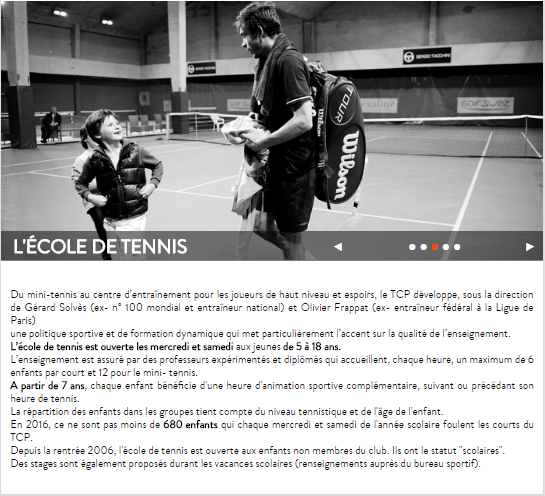
\includegraphics[scale=0.8]{1_1_expl.PNG}}
        \caption{Site avant correction de la règle 1:1}
    \end{figure}
    \newpage
    \subsubsection*{Correction de la transgression}
    Nous devrions rajouter du contenu sur certaines pages afin de leur donner un but concret.
    \begin{figure}[H]
    	\centering
        \fbox{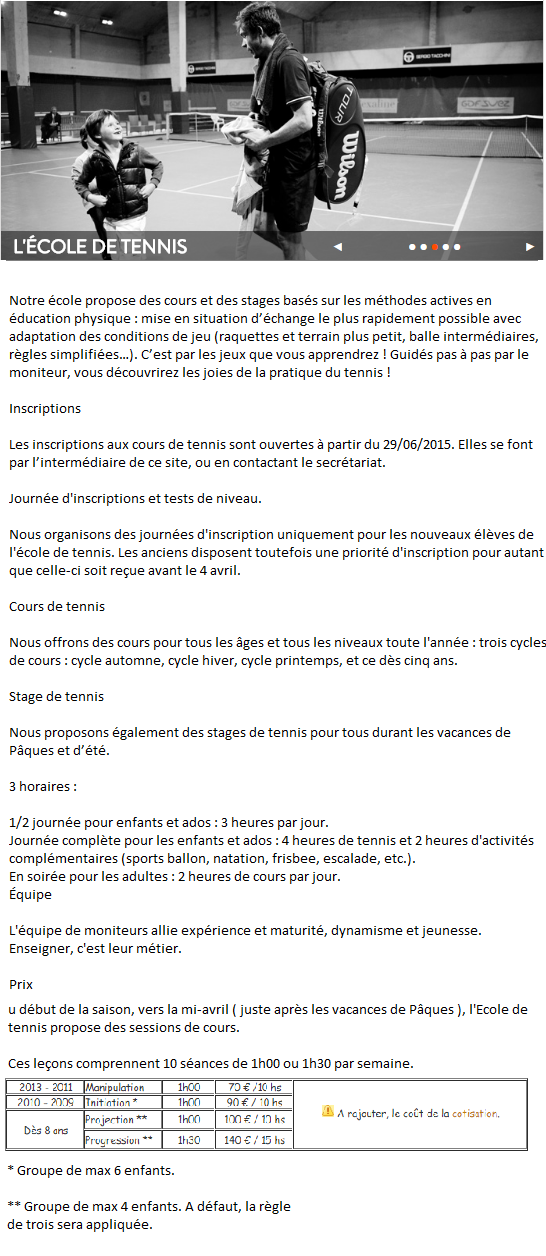
\includegraphics[width=9cm, height=16.5cm]{1_1_corr.png}}
        \caption{Site après correction de la règle 1:1}
    \end{figure}
    \begin{comment}
    \subsection{Règle 1:3 : Comprendre et répondre aux attentes de l'utilisateur }
  

      \end{comment}
     
   \subsection{Règle 2:4 : Réduire la charge de travail de l'utilisateur}
      \label{work-load}
    \begin{comment}
    \subsection{Règle 2:3 : Standardiser les séquences de tâches}
    	 \subsubsection*{Résumé de la règle}
    	 \subsubsection*{Explication de la transgression}
    	 \subsubsection*{Correction de la transgression}
    	 
   
    \subsection{Règle 2:4 : Réduire la charge de travail de l'utilisateur}}
    	 \subsubsection*{Résumé de la règle}
    	 \subsubsection*{Explication de la transgression}
    	 \subsubsection*{Correction de la transgression}
    \end{comment}
     
    \subsubsection*{Résumé de la règle}
    Allouer / Utiliser des fonctions de l'ordinateur afin de diminuer le travail de l'utilisateur.
    \subsubsection*{Explication de la transgression}
    Certaines tâches ne demandant que peu de travail via un formulaire se trouvent complexifiées via des processus actuellement devant être faits à la main au lieu d'être automatisée depuis le site Web. (Pour exemple, sur la page \href{http://www.tennisclubdeparis.fr/formule-adhesion.html}{"devenir membre"} on nous que nous devons remplir une demande d'adhésion et l'envoyer par mail afin d'attendre un retour qui sera lui même renvoyé par mail. Tout ce processus pourrait être directement effectué depuis le site web, facilitant ainsi le travail de l'utilisateur.
     \begin{figure}[H]
    	\centering
        \fbox{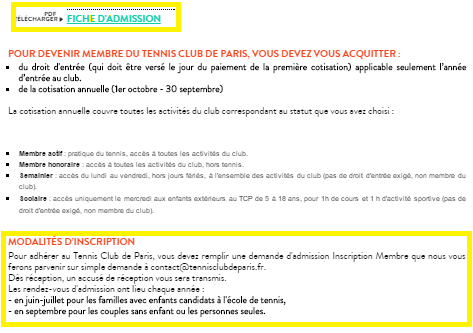
\includegraphics[scale=0.60]{2_4_expl.png}}
        \caption{Site avant correction de la règle 2:4}
    \end{figure}
    \begin{figure}[H]
    	\centering
        \fbox{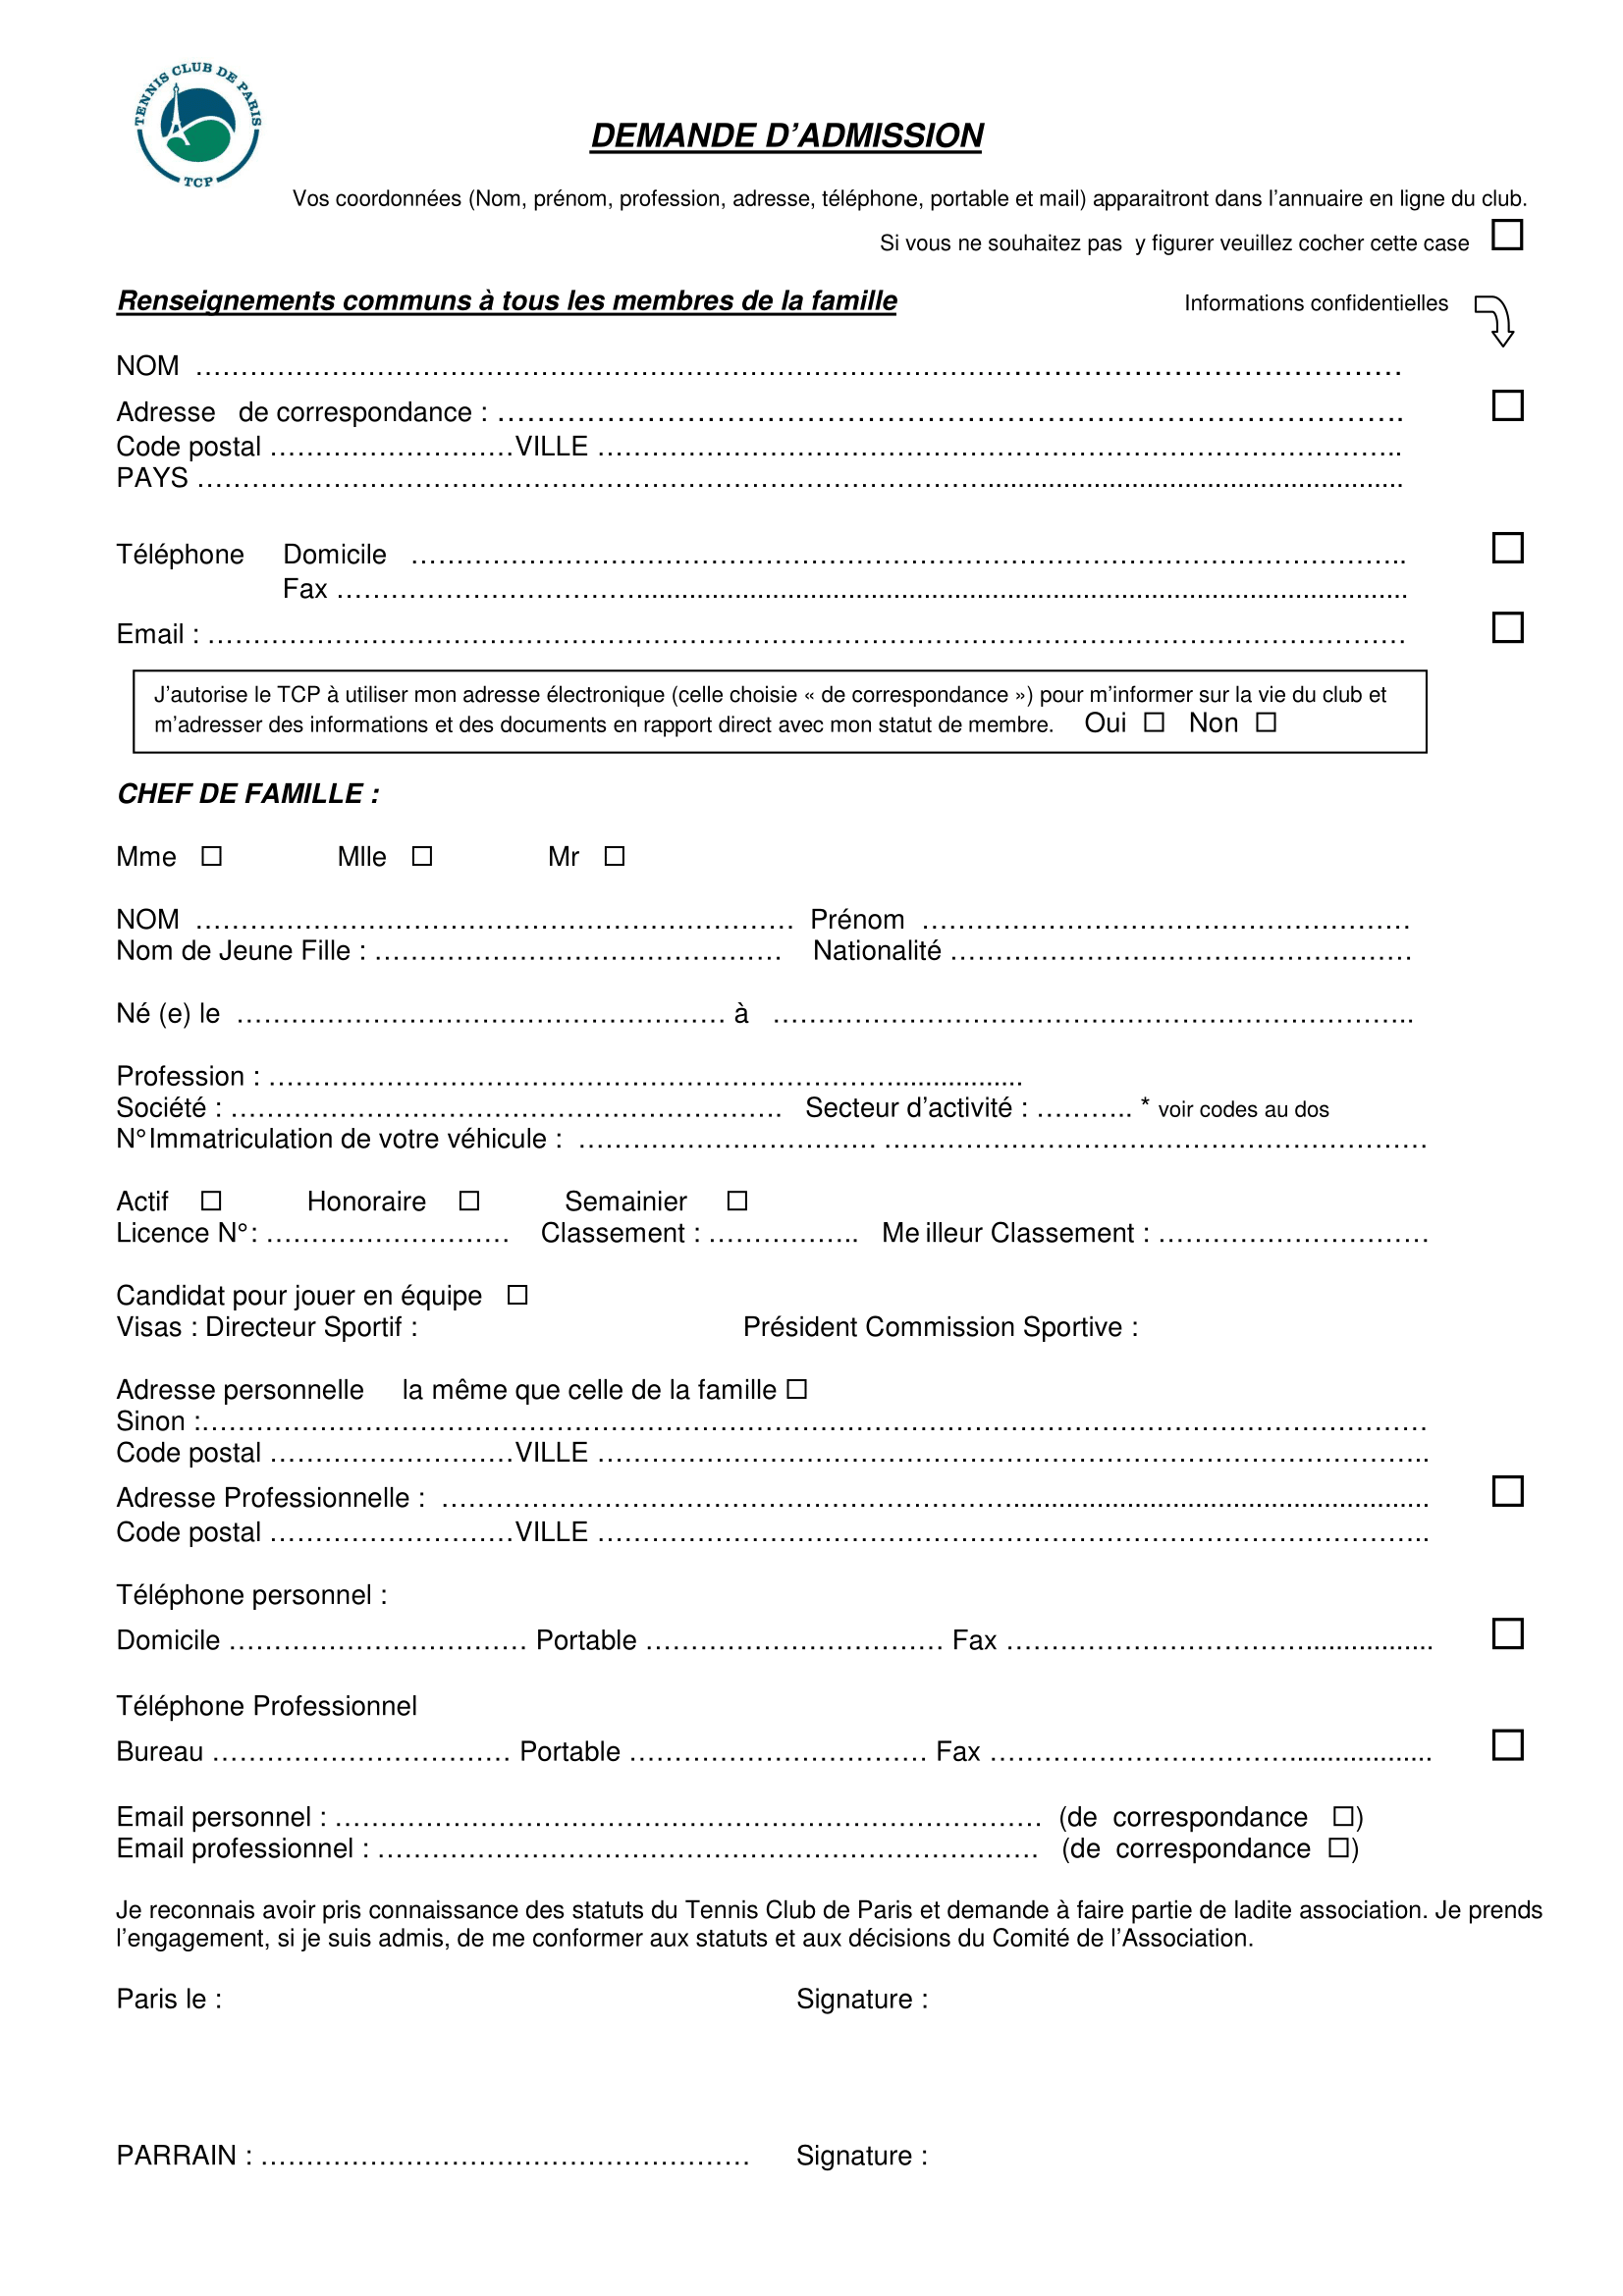
\includegraphics[scale=0.20]{fiche_admi1.png}}
        \caption{Fiche d'admission Part1}
    \end{figure}
    \begin{figure}[H]
    	\centering
        \fbox{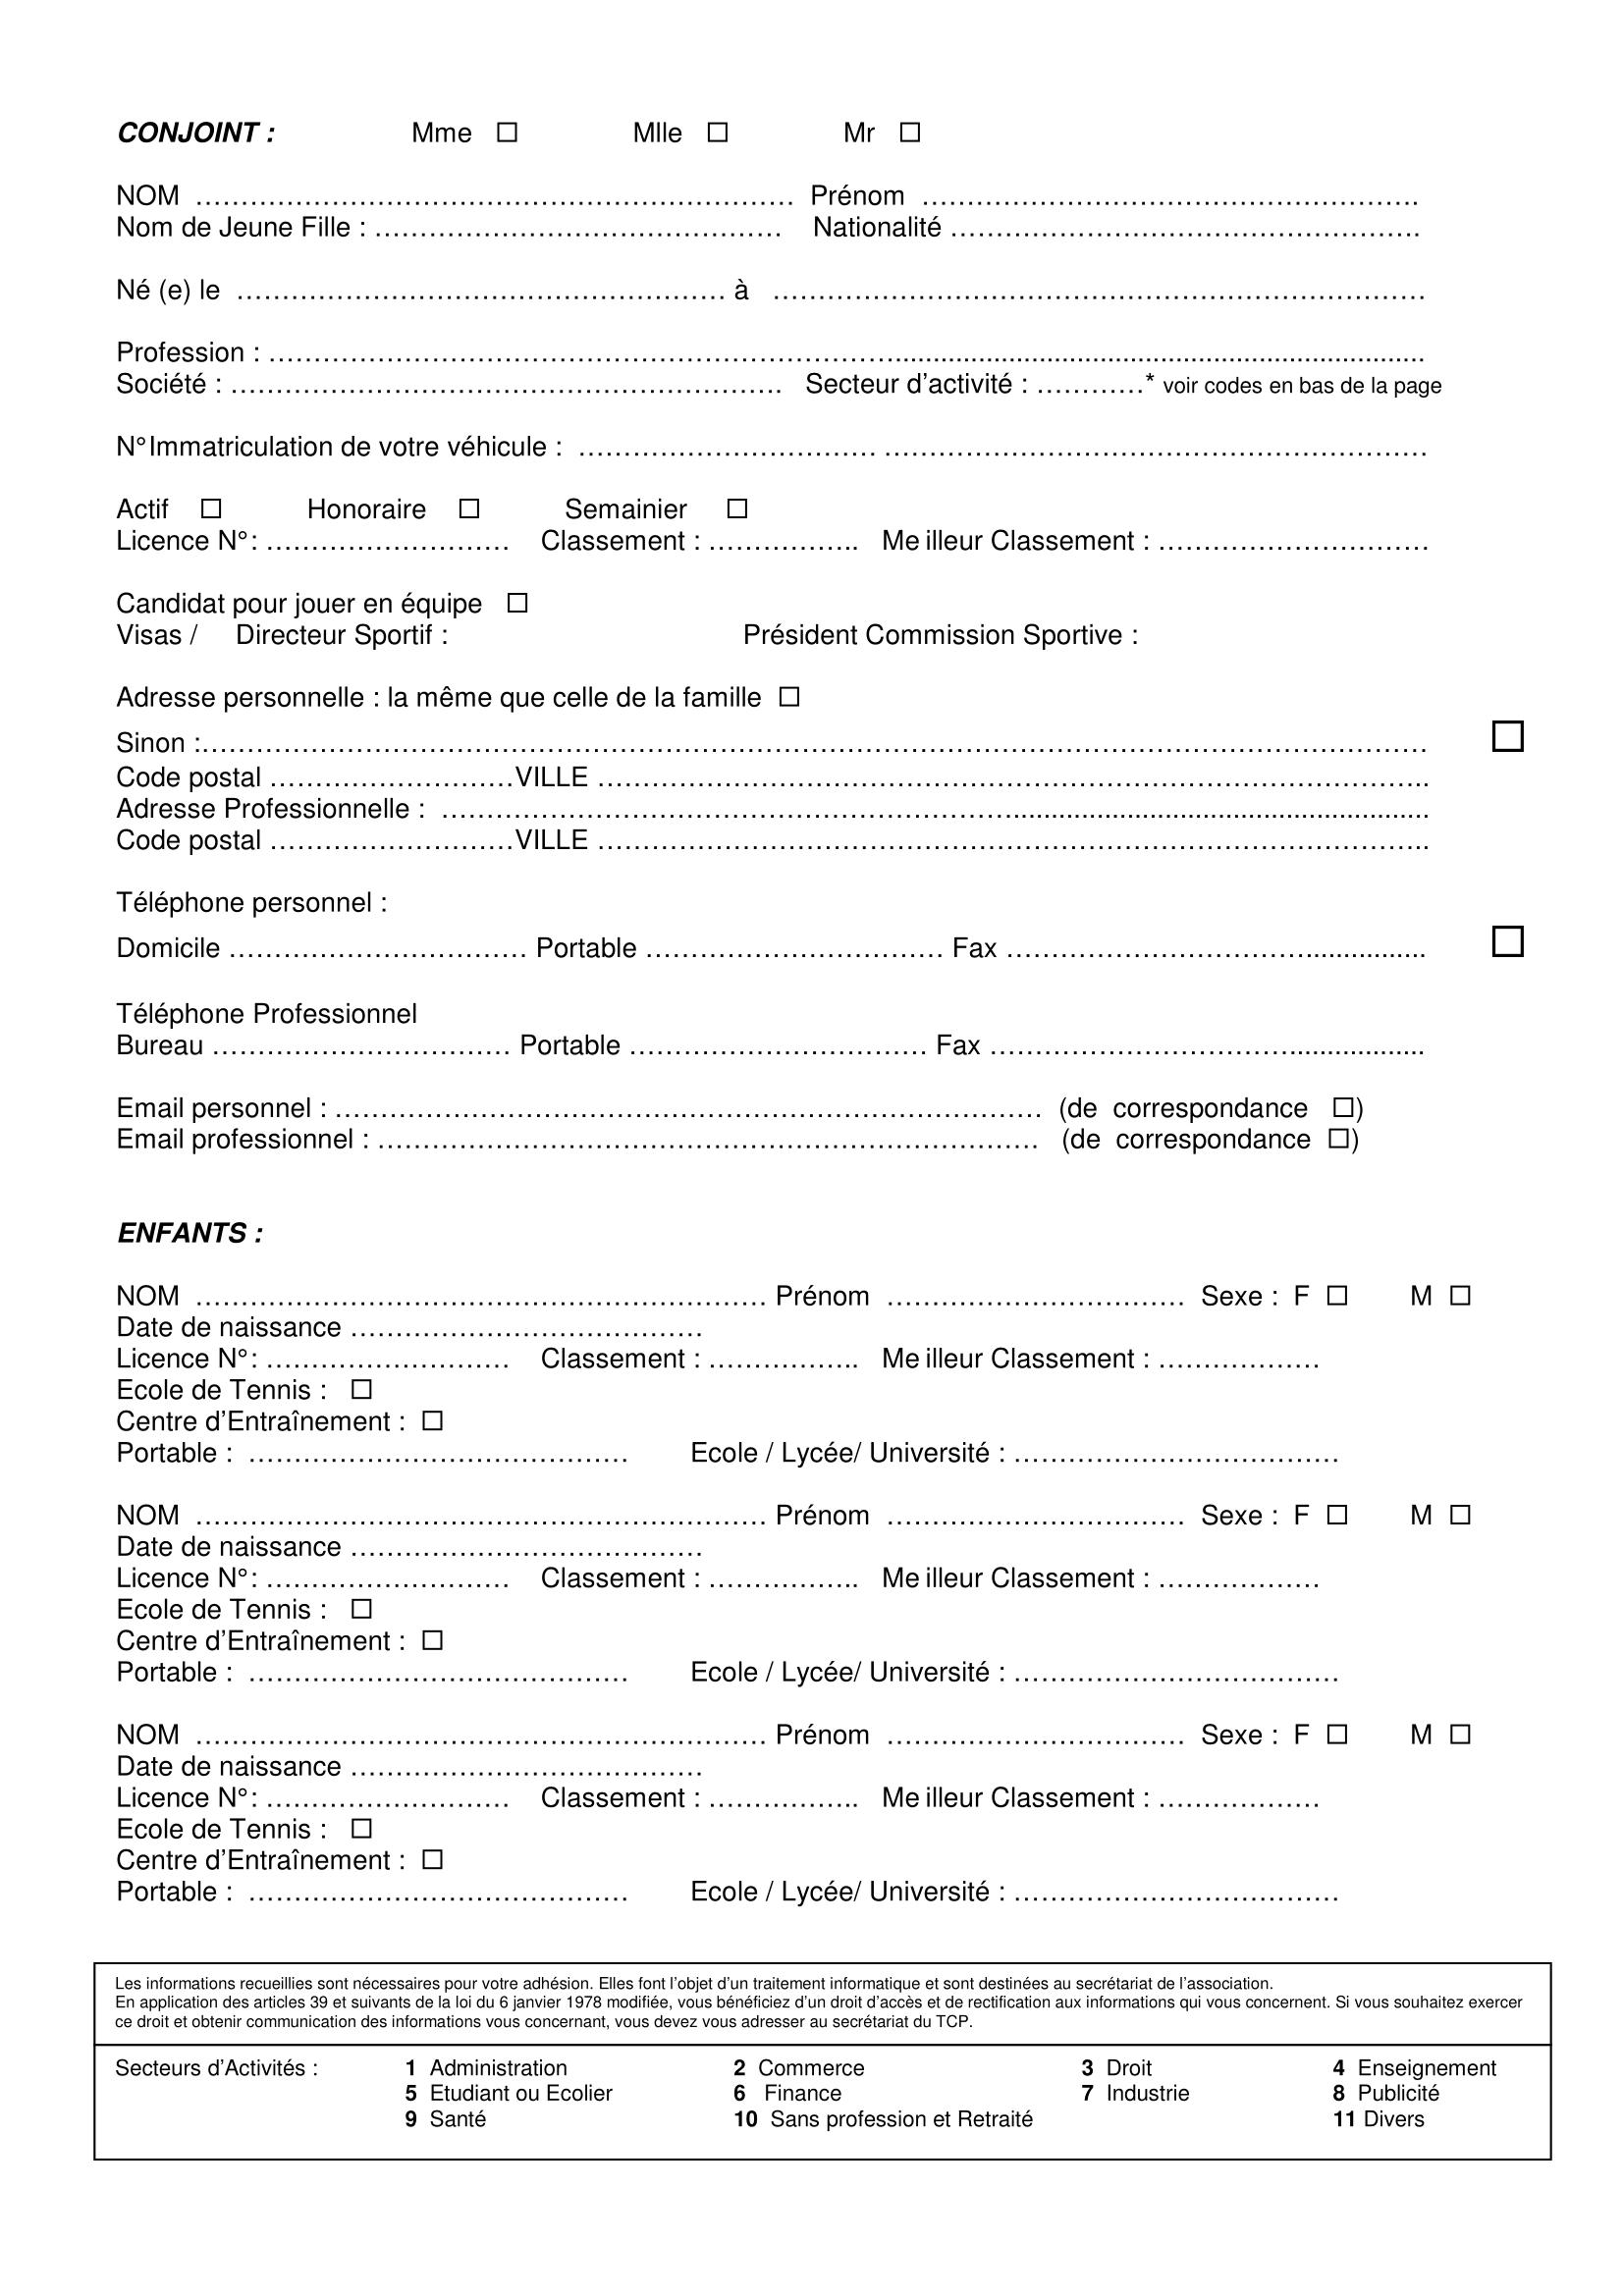
\includegraphics[scale=0.20]{fiche_admi2.png}}
        \caption{Fiche d'admission Part2}
    \end{figure}
    \subsubsection*{Correction de la transgression}
    On pourrait tout simplement automatiser certains processus afin de faciliter le travail de l'utilisateur et lui permettre d'effectuer certaines opérations directement depuis notre site Web.
     \begin{figure}[H]
    	\centering
        \fbox{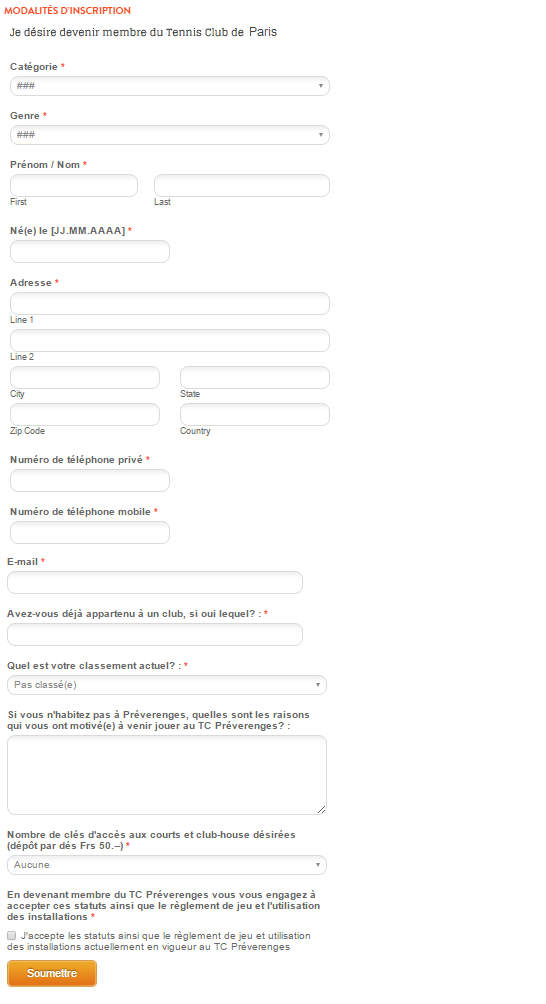
\includegraphics[scale=0.60]{2_4_corr.png}}
        \caption{Site après correction de la règle 2:4}
    \end{figure}
        \begin{comment}
    \subsection{Règle 2:5 : Concevoir en prenant en compte les limites de la mémoire de travail}

     \subsubsection*{Résumé de la règle}
     \subsubsection*{Explication de la transgression}
     \subsubsection*{Correction de la transgression}
     \end{comment}
    \subsection{Règle 6:4 : Structurer pour faciliter les comparaisons}
     \subsubsection*{Résumé de la règle}
     Structurer les pages de notre site de telle façon que des éléments supposés être comparés (afin de trouver des similarités, des différences, des tendances ou bien encore des relations) peuvent l'être le plus facilement possible. 
    \subsubsection*{Explication de la transgression}
    Sur le site du TCP, il est difficile de comparer les éléments et cela pour deux raisons : la première est tout simplement due à un manque de contenu (règle 1:1), empêchant ainsi de comparer notamment des différents événements et des différents tournois.La deuxième raison est due au fait que les infos sont parfois séparées sur différentes pages au lieu d'être regroupée au sein d'une même page.
    \newline
    \newline
    Par exemple, \href{http://www.tennisclubdeparis.fr/lecons-particulieres.html}{Les cours particuliers} et \href{http://www.tennisclubdeparis.fr/page168.html}{la recherche de partenaire} se trouvent sur deux pages différentes nous obligeant à changer de pages afin de se renseigner sur ces deux types de cours. De plus, la manque d'informations au sujet de ces deux cours nous empêche de savoir ce qui les différencie réellement.
    \begin{table}[H]
    	\centering
    	\begin{tabular}[b]{|c|c|}
    		\hline
    		\textbf{Page sur les cours particuliers} & \textbf{Page sur la recherche d'un partenaire } \\
    		\hline
    		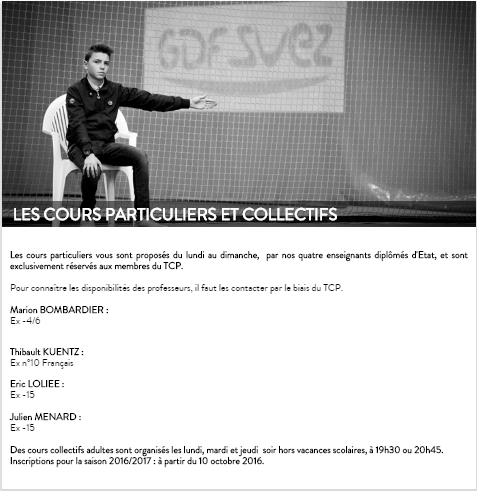
\includegraphics[width=7cm,height=9.1cm]{6_4_expl.PNG} &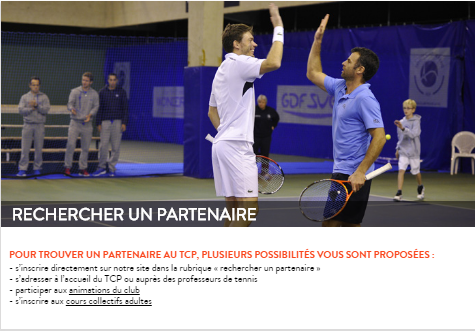
\includegraphics[width=7cm,height=9.1cm]{6_4_expl2.PNG}\\
    		\hline
    	\end{tabular}
    	\caption{Exemple de division de pages non-recommandée}
    \end{table}
\newpage
    \subsubsection*{Correction de la transgression}
    Nous pouvons regrouper certaines infos présentes à divers endroits et rajouter du contenu comme précisé dans la règle 1:1.
    \begin{figure}[H]
    	\centering
        \fbox{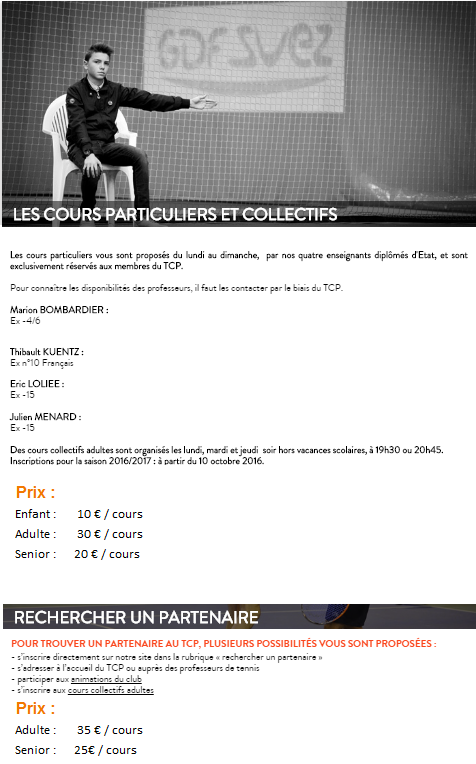
\includegraphics[width=10cm,height=15cm]{6_4_corr.png}}
        \caption{Page sur la recherche d'un partenaire}
    \end{figure}
    
     \subsection{Règle 7:6 : Utiliser des labels d'onglets cohérents}
     \label{label_coherent}
    \subsubsection*{Résumé de la règle}
   Le site doit comporter des labels qui sont clairement descriptif de leur fonction ou de leur destination.
    \subsubsection*{Explication de la transgression}
    Sur le site choisis, de nombreux labels portent à confusion, notamment ceux-de la barre de navigation. Le label "événements" pour exemple comporte un lien vers la salle de fitness du TCP (Ce lien s'appellent lui même "Au TCP, "TOQP""). Ceci peut parfois porter l'utilisateur à confusion. 
    \begin{figure}[H]
    	\centering
        \fbox{
\includegraphics{7_6_expl.png}}
        \caption{Label menant à la page sur la salle de fitness}
    \end{figure}

    \subsubsection*{Correction de la transgression}
    Remplacer certains nom de label peu explicite en d'autres plus explicite.
     \begin{figure}[H]
    	\centering
        \fbox{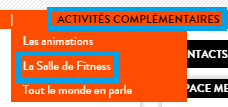
\includegraphics{7_6_corr.PNG}}
        \caption{Correction suite à la règle 7:6}
    \end{figure}
  \newpage
    \subsection{Règle 10:2 : Proposer des liens vers du contenu relatif}
    \subsubsection*{Résumé de la règle}
    Le site doit comporter des liens vers d'autres pages web ayant du contenu en relation avec celui présent sur notre site.
    \subsubsection*{Explication de la transgression}
    Nous nous sommes mis à la place d'un joueur professionnel jouant dans ce club qui voudrait connaître son score au niveau nationale, avoir des informations sur le fédération de tennis, .... Le site manque de liens vers du contenu extérieur, nous ne trouvons que les liens vers les sponsors.
        \begin{figure}[H]
        	\centering
        	\fbox{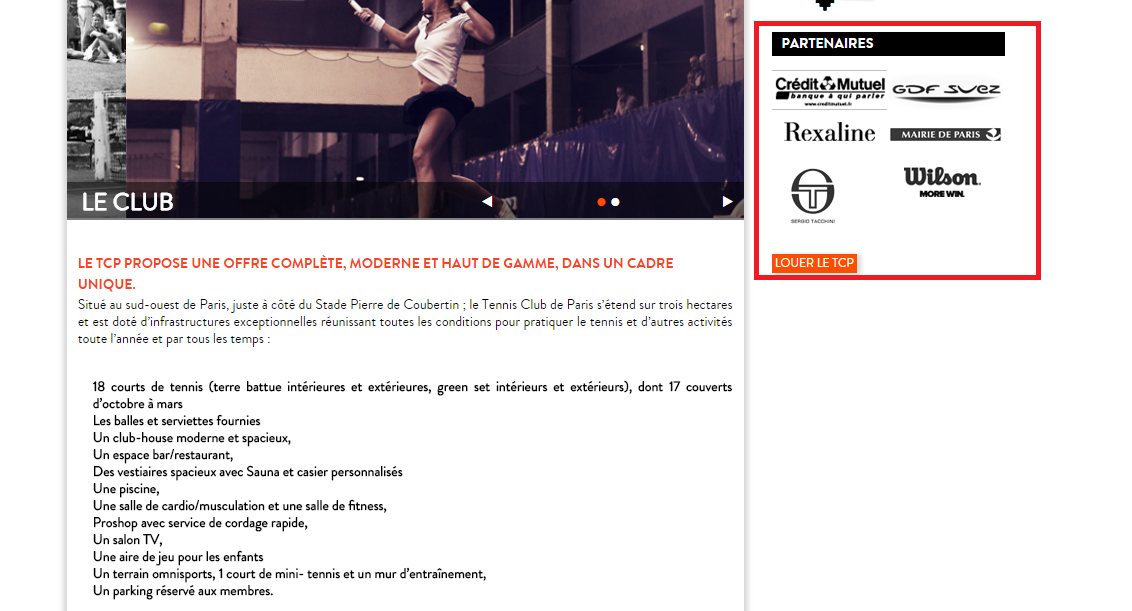
\includegraphics[width=\textwidth,height=4cm]{10_2_expl.png}}
        	\caption{Les liens proposés sont uniquement des sponsors commerciaux.}
        \end{figure}
    
    \subsubsection*{Correction de la transgression}
    Il faudrait ajouter quelques liens extérieures utiles en rapport avec le tennis, la compétition, etc.
        \begin{figure}[H]
        	\centering
        	\fbox{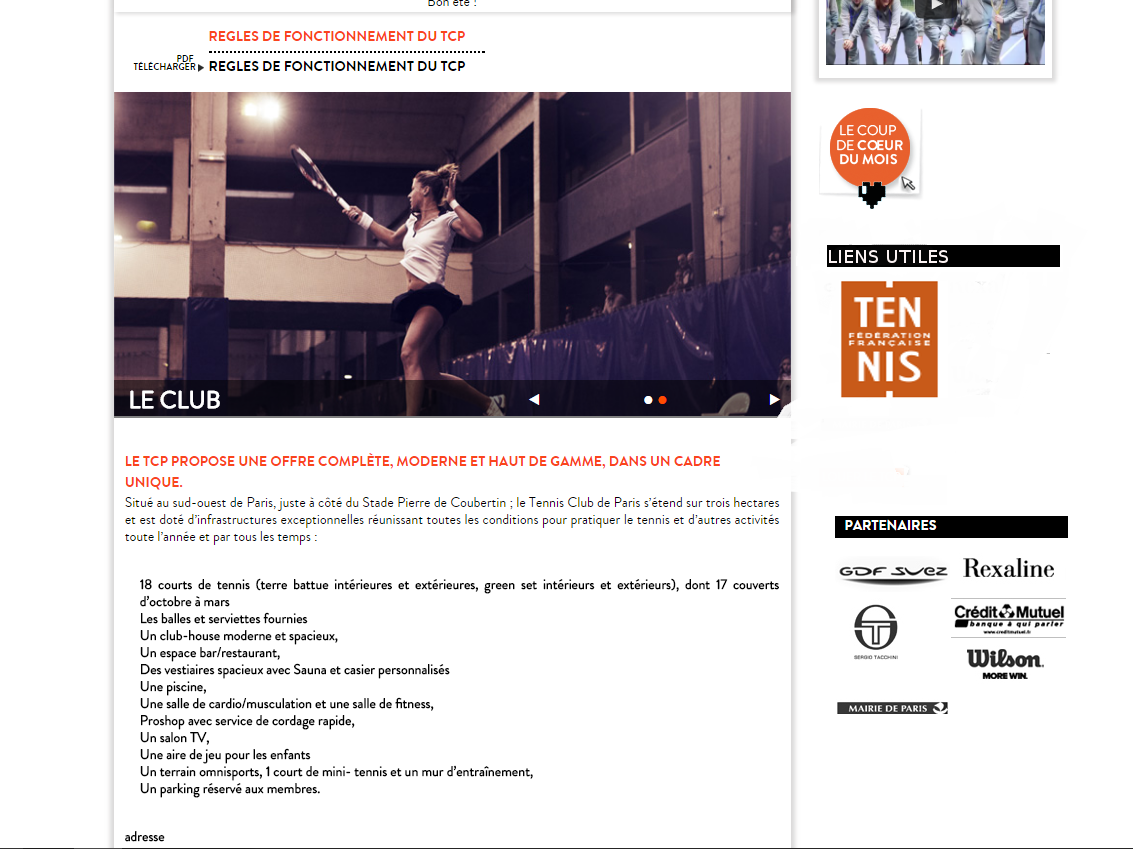
\includegraphics[width=\textwidth,height=4.5cm]{10_2_corr.PNG}}
        	\caption{Correction suite à la règle 10:2}
        \end{figure}
   \newpage
    \subsection{Règle 14:3 : S'assurer que les images ne ralentissent pas le téléchargement de la page}
   \subsubsection*{Résumé de la règle}
   Assurer vous que les images présentes sur votre site web ne ralentissent pas plus que nécessaire le temps de chargement de la page.
   \subsubsection*{Explication de la transgression}
   Sur le site de nombreuses images sont présentes, voire même un peu trop nombreuse, cela impacte directement la vitesse de chargement et en plus de cela recouvre une grande partie de la page.
   \begin{figure}[H]
   	\centering
   	\fbox{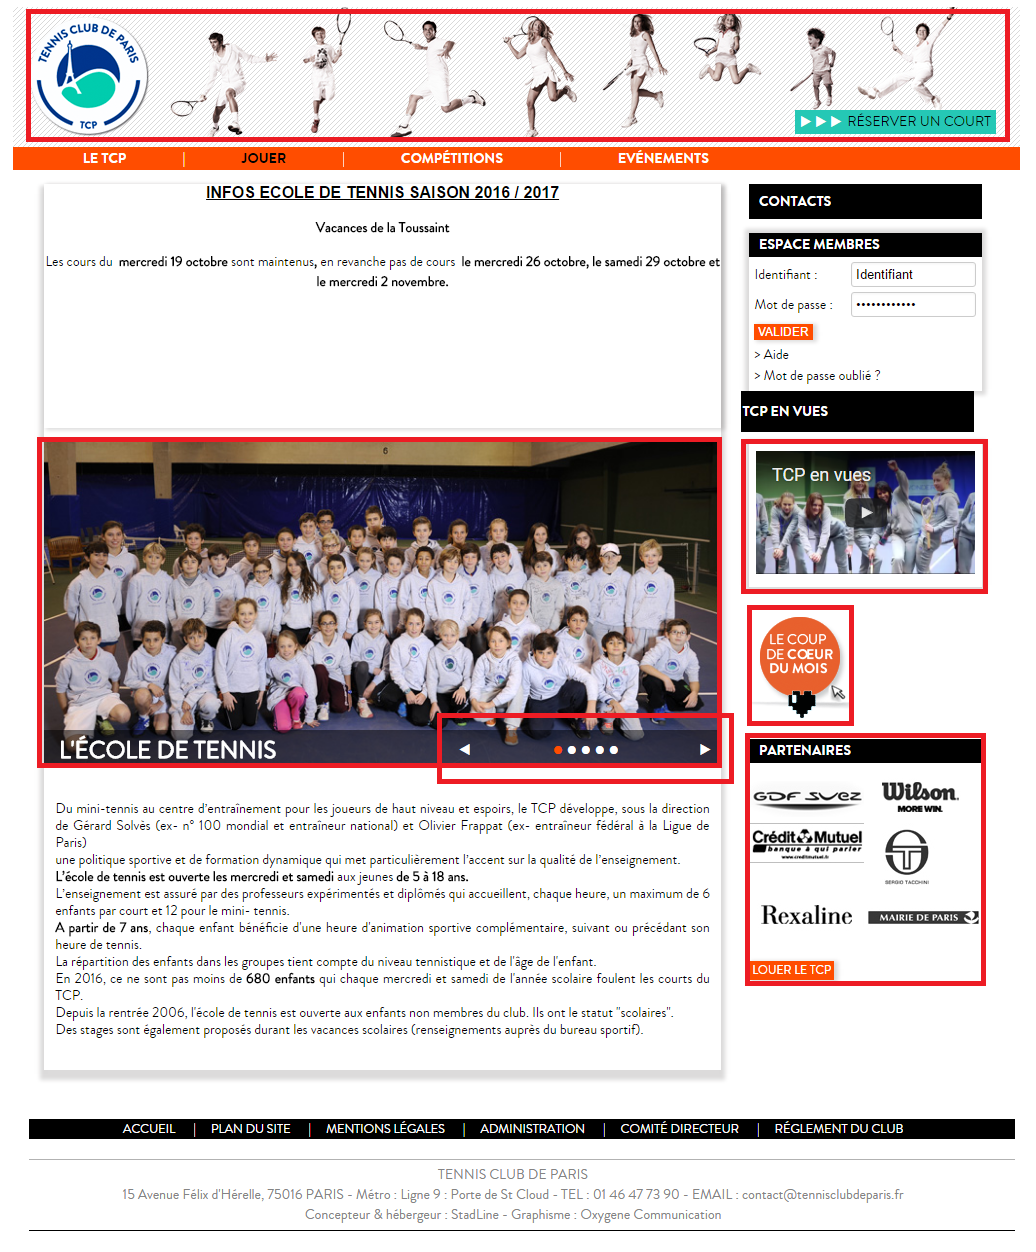
\includegraphics[width=10cm, height=12cm]{14_3_expl.PNG}}
   	\caption{Constat du nombres d'images sur la page}
   \end{figure}
   \subsubsection*{Correction de la transgression}
   Supprimer les images superflues, afin de favoriser les performances, quitte à perdre un peu du design de notre site. Il faut néanmoins trouver un juste milieu et donc conserver le design du site tout en permettant une amélioration des performances.
   \begin{figure}[H]
   	\centering  \fbox{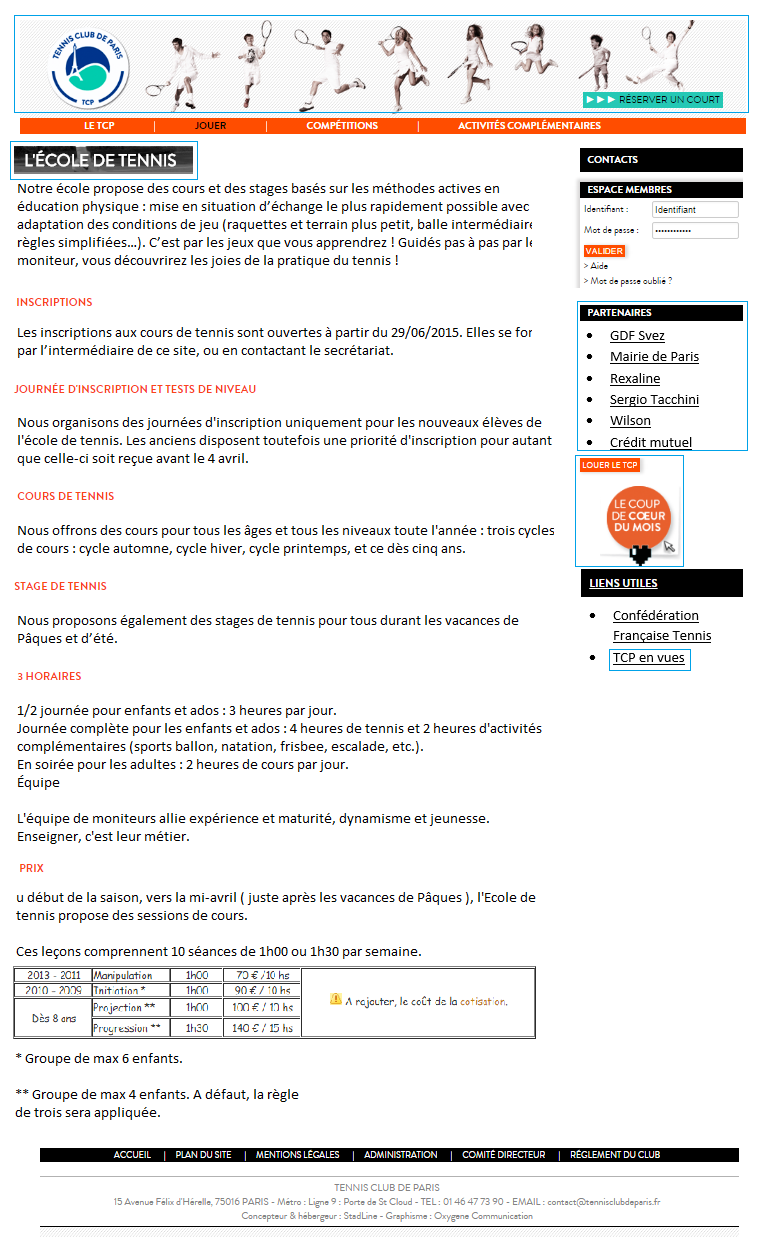
\includegraphics[width=10cm, height=15cm]{14_3_corr.png}}
   	\caption{Site après suppression d'images superflues}
   \end{figure}
   
   \subsection{Règle 14:4 : Utiliser les vidéos, les animation et l'audio de manière sensée}
    	    \subsubsection*{Résumé de la règle}
	    	Les videos, animation et audio devraient être utilisés seulement pour transmettre le message du contenu du site. Ceux-ci peuvent se montré distrayant pour l'utilisateur. De plus ceux-ci ralentissent le chargement de la page, ils doivent en valoir la peine. S'ils sont bien  utilisés, les greffons multimédia peuvent améliorer l'expérience utilisateur.
    	    
    	    \subsubsection*{Explication de la transgression}
    	       Sur le site, on compte pas moins de 5 diaporamas qui reprennent des photos de décoration qui ne permettent de pas de mieux comprendre le contenu de la page (des photos de personnes qui jouent au tennis, qui prennent la pose, etc). 
    	       \begin{figure}[H]
    	       	\centering
    	       	\fbox{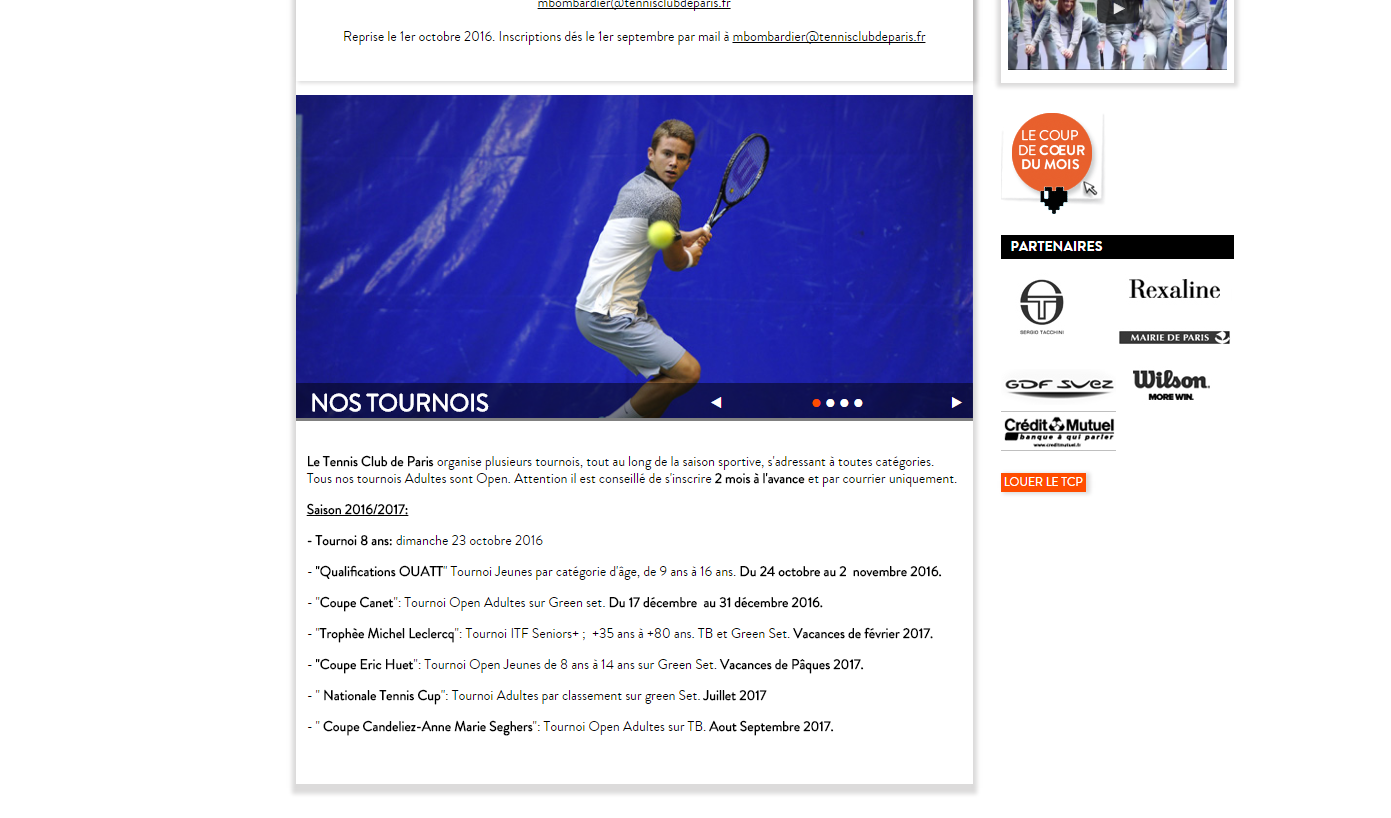
\includegraphics[width=\textwidth, height=10cm]{14_4_expl.PNG}}
    	       	\caption{Diaporama non-essentiel qui distrait le lecteur}
    	       \end{figure}
    	    \subsubsection*{Correction de la transgression}
	    	    Le site ayant prévu une section  \href{http://www.tennisclubdeparis.fr/album-photo.html}{"Le TCP en vues"} regroupant différents albums photos, nous recommanderions à la personne en charge du design de limiter ces animations photographique quitte à prévoir une zone pour les diaporamas dans la section prévue à cet effet.
	    	      \begin{figure}[H]
	    	      	\centering
	    	      	\fbox{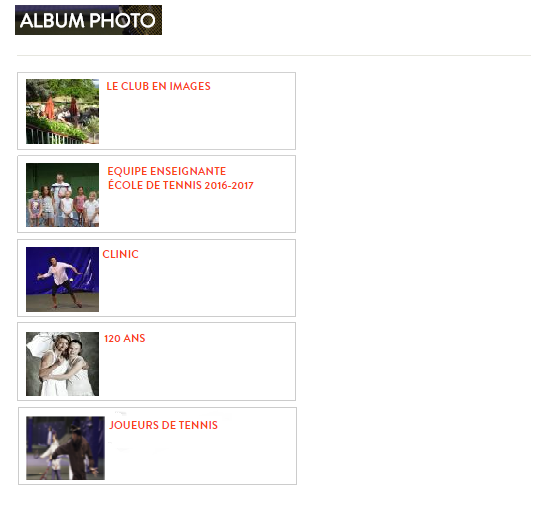
\includegraphics[width=\textwidth, height=6.5cm]{14_4_corr.PNG}}
	    	      	\caption{Les diaporamas non-essentielles sont placées sur la page "Album photos" (TCP en vue)}
	    	      \end{figure}
	   \begin{comment}
	   double emploi avec 14:4	    
    \subsection{14:7 Limit Large Images Above the Fold}
    \subsubsection*{Résumé de la règle}
    \subsubsection*{Explication de la transgression}
    \subsubsection*{Correction de la transgression}
	\end{comment}

    \subsection{Règle 15:6 : Utiliser des casses différentes dans la prose}
    \subsubsection*{Résumé de la règle}
    Afficher le texte continu (prose) en utilisant des lettres mixtes majuscules et minuscules.L'utilisation de majuscules doit être utilisée pour indiquer de début d'une phrase, avec es noms propres ou encore avec des acronymes. Si l'on désire attirer l'attention de l'utilisateur on mettra la partie désirée en gras, en italique ou entièrement en majuscules.
    	\newpage
    \subsubsection*{Explication de la transgression}
    Cette règle est surtout transgressée sur une page du site : \href{http://www.tennisclubdeparis.fr/historique.html}{L'Histoire du TCP}. Sur cette dernière, l'entièreté des noms propres sont entièrement en majuscules. Cela ralentit fortement la lecture et a tendance à attirer le regard de l'utilisateur.
    \begin{figure}[H]
    	\centering  \fbox{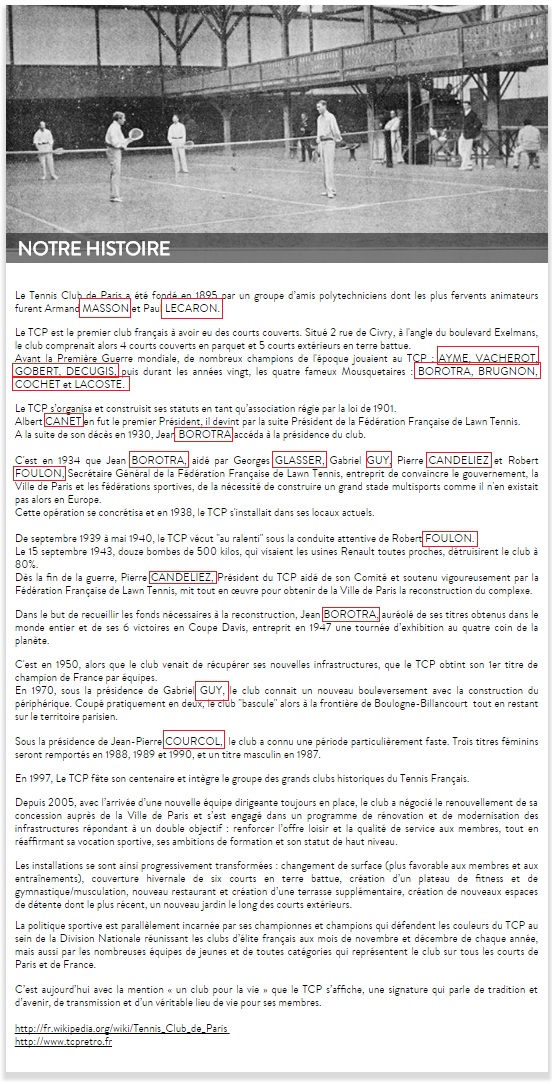
\includegraphics[width=8cm, height=16cm]{15_6_expl.png}}
    	\caption{Constat du nombre de nom propre entièrement en majuscules}
    \end{figure}
    \subsubsection*{Correction de la transgression}
    Ne mettre en majuscule que la première lettre du nom propre, permettant ainsi à l'utilisateur d'être plus à l'aise sur le site tout en permettant les noms propres de se démarquer légèrement du reste du texte.
    \begin{figure}[H]
    	\centering  \fbox{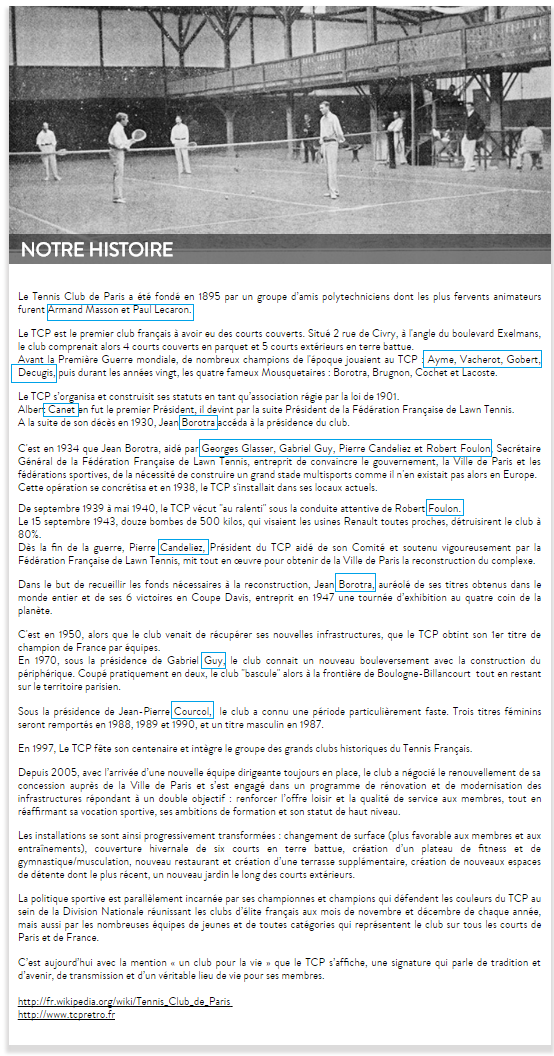
\includegraphics[width=10cm, height=16cm]{15_6_corr.png}}
    	\caption{Site après la modification des noms propres}
    \end{figure}
    \subsection{Règle 16:3 : S'assurer que l'information nécessaire soit affichée }
     \subsubsection*{Résumé de la règle}
  Il faut dans le site que toutes les informations nécessaires soient affichées.
     
     \subsubsection*{Explication de la transgression}
     Le règlement du club n'est pas présent sur le site. Un \href{http://www.tennisclubdeparis.fr/reglement.html}{lien}  y mène mais sans rien afficher 
    
     \begin{figure}[H]
     	\centering
     	\fbox{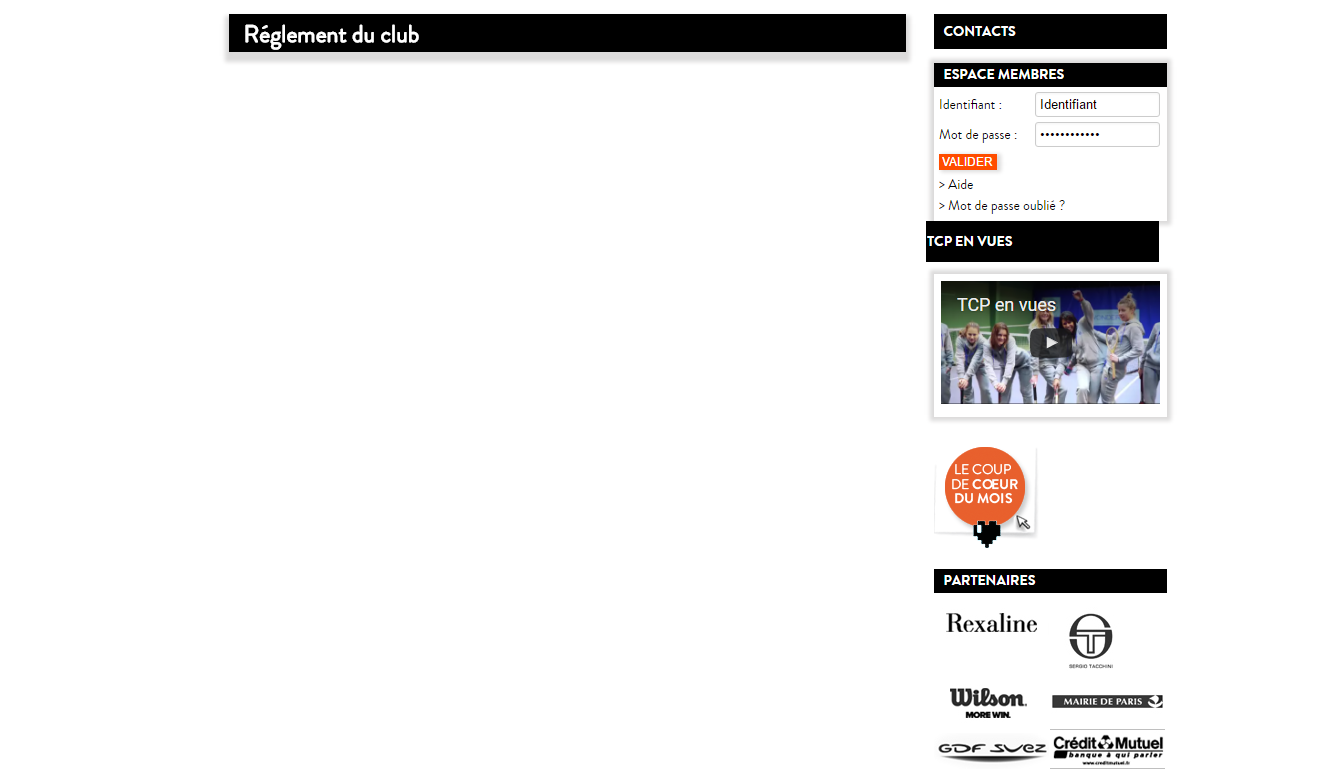
\includegraphics[width=\textwidth, height=8cm]{16_3_expl.PNG}}
     	\caption{Réglement du club vide}
     \end{figure}
     \newpage
     \subsubsection*{Correction de la transgression}
    Il faudrait inclure le règlement sur la page prévue à cet effet.
     \begin{figure}[H]
     	\centering
     	\fbox{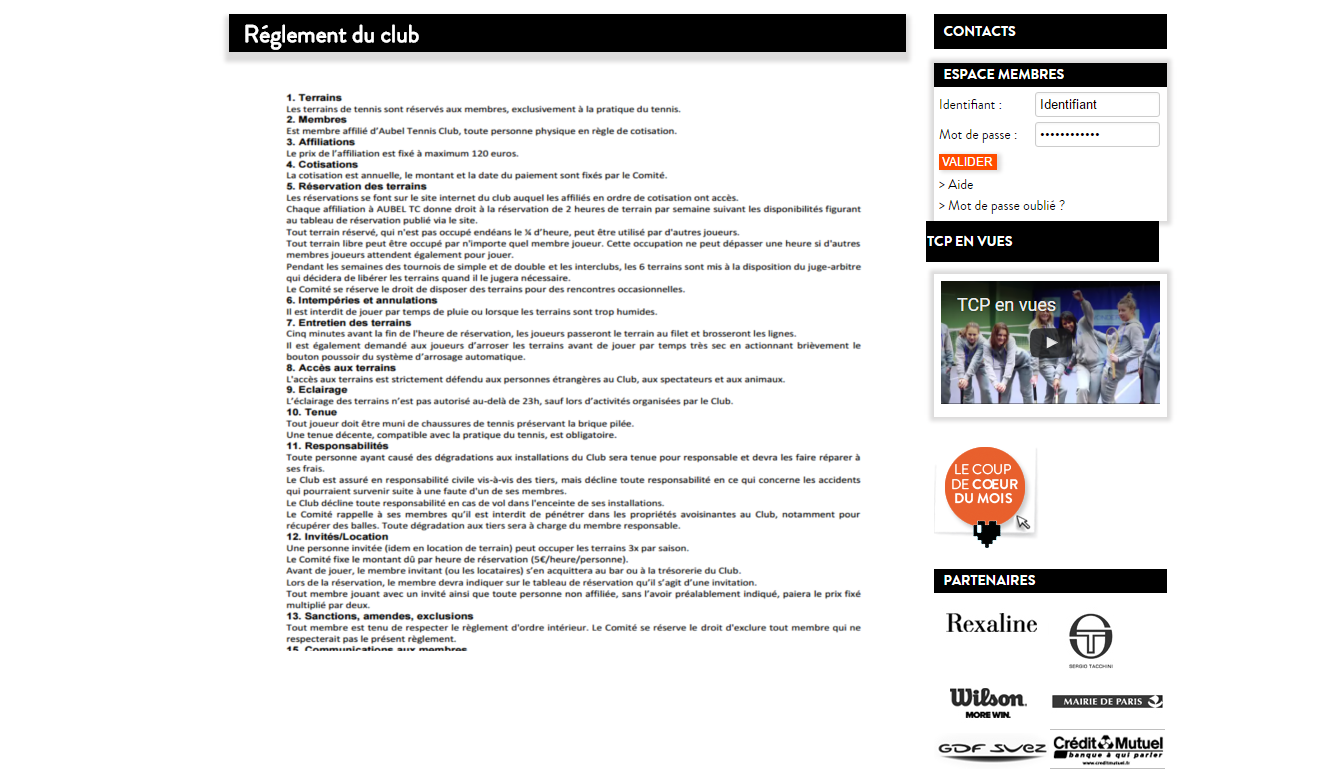
\includegraphics[width=\textwidth, height=9cm]{16_3_corr.PNG}}
     	\caption{Les photos non-essentielles sont placées sur la page "Album photos" (TCP en vue)}
     \end{figure}
     \begin{comment}
    \subsection{Règle 16:8 : Formater l'information pour des audiences diverses}
    \subsubsection*{Résumé de la règle}
Le site doit pouvoir fournir l'information dans de différents formats si celui-ci possède différentes audiences intéressées par la même information.
    \subsubsection*{Explication de la transgression}
    \subsubsection*{Correction de la transgression}
    \end{comment}
    \section{Source}

    SCHEIDERMAN B et LEAVITT 0.M. \textit{Research-Based Web Design \& Usability Guidelines.} GSA.  Washigton, USA.
    
\end{document}

